%!TEX root = ../main.tex
% !TeX encoding = UTF-8
\section{Helmet Prototype for Cyclist Safety} \label{chap:prototipo}

    %Neste trabalho foi desenvolvido um protótipo de capacete no qual realizaria verificações de distância de objetos nas costas do ciclista, alertando-o de possíveis riscos de acidentes.
    %Caso esteja em situação de risco, o capacete emitiria sinais visuais luminosos, além do envio de aviso para um segundo dispositivo como um \textit{smartphone} alertando de sua situação.
    In this work was developed a prototype of the helmet which performs verification of distance of objects on the back of the cyclist, alerting him of potential risks of accidents.
    If he is in the risk situation, the helmet will send luminous visual signals, beyond of to send the warning to a second device like a smartphone also.
    

    \subsection{Call Graph and Partitioning Candidate Codes}
        
        %Como é exibido na Figura \ref{fig:gc}, o grafo de chamada do \wearable\ constitui-se basicamente de leitura das distâncias, cálculo de risco e aviso ao usuário.
        % o que é iteração do wearable
        %Cada ciclo é considerado uma iteração do sistema \wearable.
        As is shown in Figure~\ref{fig:gc}, the call graph of wearable is basically of distances checks, calculate of risk and warning to the user.
        Each cycle is considered one iteration of the wearable system.
        
        \begin{figure}[h] \centering
            \vspace{-0.5em}
            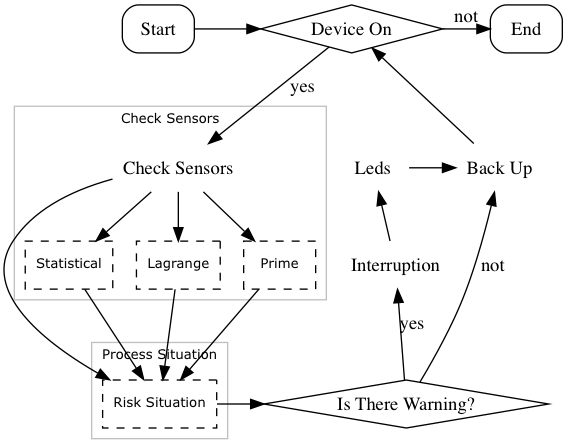
\includegraphics[width=0.45\textwidth]{img/capacete.png}
            \caption{Algorithm call graph of wearable base. Grid items display the location of partitioning algorithms.}
            \label{fig:gc}
        \end{figure}
        
        %O particionamento foi avaliado em duas seções principais, sendo elas a de leitura e de processo de situações, constituindo-se de quatro situações diferentes de particionamento para análise (itens pontilhados na Figura \ref{fig:gc}).
        The partitioning was evaluated in two main sections, mean them the check of distance and situations processing, constituting of four different situations of partitioning for analyzing (items dotted in Figure~\ref{fig:gc}).
        
        %Os algoritmos \A$_{i}$\ candidatos ao particionamento serão:
        The candidate algorithms \A$_{i}$\ to the partitioning was:
        
        \begin{itemize}
            %\item \A$_{St}$: Análise Estatística (Algoritmo \ref{alg:statistic}) calculará valores de desvio padrão e variância dos valores no \buffer;
            \item \A$_{St}$: Statistical Analysis (Algorithm \ref{alg:statistic}) will calculate the standard derivation and variance of the buffer's values;
            
            %\item \A$_{La}$: Lagrange (Algoritmo \ref{alg:lagrange}) interpolará novas distâncias a partir dos dados do \buffer; 
            \item \A$_{La}$: Lagrange (Algorithm \ref{alg:lagrange}) will interpolate new distances by buffer's values;
            
            %\item \A$_{PN}$: Números Primos (Algoritmo \ref{alg:prime}) avaliará se a soma das distâncias lidas correspondem aos números primos;
            \item \A$_{PN}$: Prime Numbers (Algorithm \ref{alg:prime}) will evaluate if the sum of distances read correspond to a prime number;
            
            %\item \A$_{Ri}$: Processamento de risco (Algoritmo \ref{alg:risk}), na seção de processo de situações.
            \item \A$_{Ri}$: Risk Processing (Algorithm \ref{alg:risk}), in section of situation process.
        \end{itemize}
    
    
        %!TEX root = ../main.tex
% !TeX encoding = UTF-8

       \begin{algorithm}[t] \footnotesize
           \KwIn{buffer vector.}
           \KwOut{mean, variance, standard derivation.}
           
           \BlankLine
           \Begin{
               $\vars{sum}= \vars{variance} = 0$;
               \BlankLine
               
               \lFor{$\func{length}(\vars{buffer})$}{$\vars{sum} \mathrel{+}= \vars{buffer}_i$}
               \BlankLine
               
               $\vars{mean} = \vars{sum} \div \func{length}(\vars{buffer})$\;
               \BlankLine
               
               
               \lFor{$\func{length}(\vars{buffer})$}{
                   $\vars{variance} \mathrel{+}= (\vars{buffer}_i - \vars{mean})^2$
               }
               
               \BlankLine
               $\vars{variance} \mathrel{\div}= \func{length}(\vars{buffer})$\;
               \BlankLine
               $\vars{sd} = \func{sqrt}(\vars{variance})$\;
               
               \Return \vars{mean}, \vars{variance}, \vars{sd}\;
           }
           \caption{Statistical Method.}
           \label{alg:statistic}
       \end{algorithm}
       
       \begin{algorithm}[b] \footnotesize
           \KwIn{buffer vector, point.}
           \KwOut{interpolated distance.}
           
           \BlankLine
           \Begin{
               
               $\vars{new\_distance} = 0$\;
               \BlankLine
               
               \For{$\vars{i}\ in\ 1:\func{length}(\vars{buffer})$}{
                   $\vars{c} = \vars{d} = 1$;
                   
                   \BlankLine
                   \For{$\vars{j}\ in\ 1:\func{length}(\vars{buffer})$}{
                       \If{$\vars{i} \ne \vars{j}$}{
                           $\vars{c} \mathrel{\times}= \vars{point} - \vars{j}$;
                           %\BlankLine
                           $\vars{d} \mathrel{\times}= \vars{i} - \vars{j}$;
                       }
                   }
                   \BlankLine
                   $\vars{new\_distance} \mathrel{+}= \vars{buffer}_i \times \vars{c} \div \vars{d}$;
               }
               \BlankLine
               
               \lIf{$\vars{new\_distance} \ge 0$}{$\Return\ \vars{new\_distance}$}
               \lElse{$\Return\ 0$}
               
           }
           \caption{Interpolation by Lagrange Method.}
           \label{alg:lagrange}
       \end{algorithm}
       
       \begin{algorithm}[t] \footnotesize
           \KwIn{distance$_1$, distance$_2 = 0$, distance$_3 = 0$.}
           \KwOut{primacy.}
           
           \BlankLine
           \Begin{
               
               $\vars{prime} = \vars{distance}_1 + \vars{distance}_2 + \vars{distance}_3$;
               \BlankLine
               
               \lIf{$\vars{prime} \le 1$}{\Return 0}
               \BlankLine
               \lIf{$\vars{prime} = 2$}{\Return 1}
               \BlankLine
               
               \lIf{\vars{prime} $\func{mod}(2) = 0$}{$\vars{prime} \mathrel{+}= 1$}
               \BlankLine
               
               $\vars{divider} = \vars{prime} \div 2$;
               
               \lIf{\vars{divider} $\func{mod}(2) = 0$}{$\vars{divider} \mathrel{+}= 1$}
               \BlankLine
               
               
               \While{\vars{divider} $> 2$}{
                   \lIf{\vars{prime} $\func{mod}(divider) = 0$}{\Return 0}
                   \BlankLine
                   \lElse{\vars{divider} $\mathrel{-}= 2$;}
                   
               }
               \Return 1;
               
           }
           \caption{Prime Number Method.}
           \label{alg:prime}
       \end{algorithm}
       
       \begin{algorithm}[b]
           \footnotesize
           \KwIn{distance read; min distance.}
           \KwOut{boolean.}
           
           \BlankLine
           \Begin{
               \tcp{If there is risk, return TRUE}
               \uIf{\vars{distance\_read} $\le$ \vars{min\_distance}}{
                   \Return 1
               }
               \lElse {
                   \Return 0
               }
               
           }
           \caption{Risk Processing Method.}
           \label{alg:risk}
       \end{algorithm}
       
        
        %Explicando as implementações de A
        %Foi realizado o particionamento para cada algoritmo candidato \A$_{i}$, gerando tanto sua versão em código em nível de \software,\ quando seu módulo em \hardware,\ utilizados para testes comparativos de desempenho.
        It was made the partitioning for each candidate algorithm \A$_{i}$, building both its software level code version and its hardware module, both used for comparative tests.
        
        % s de forma geral
        %Para a execução dos testes, todos os \A$ _i $\ em suas versões \hs\ foram executados em implementações sistêmicas sintetizáveis \Ss$ _j $,\ constituídas de módulos como \textit{soft-}processador MicroBlaze, além de memórias, interfaces para comunicação com os dispositivos conectados, entre outros, permitindo o funcionamento completo do \wearable\ \cite{obeidat2011microblaze}.
        For the execution of the tests, all the \A$ _i $\ in its hardware and software versions ran in synthesizable systemic implementations \Ss$ _j $,\ constituted of modules as MicroBlaze soft-processor, beyond of memories, interfaces for communication with the connected devices, among others, allowing the full operation of wearable \cite{obeidat2011microblaze}.
        
        % as versões de a em software
        %Todos os algoritmos \A$_{i}$ em suas versões de \software\ foram executados em uma única implementação \Ss$ _j $, já que esta era compatível com qualquer aplicação em nível de \software, dependendo somente da disposição das instruções na memória.
        %Ou seja, para trocar o \A$_{i}$ por \A$_{k}$ neste sistema basta recompilar o projeto em \software.
        %Os testes neste sistema serão referenciados como \Ss$ _{s} $.
        All the algorithms \A$ _i $\ in its software versions ran in one unique \Ss$ _j $ implementation, since it was compatible with any application in software level, depending only on the availability of instructions in its memory.
        In other words, to change the \A$ _i $ to \A$ _k $ in this system need to recompile the project in software.
        The tests in this system will be referenced as \Ss$ _{s} $.
        
        % algoritmos em hardwares
        % explicando que a necessitam de interfaces
        %Algoritmos \A$ _i $\ em \hardware\ também executam em sistemas \Ss$ _j $, mas tais sistemas possuem características ímpares já que são acrescentados módulos sintetizáveis de cada algoritmo.
        %
        %Como cada \A$_i$ possui seu próprio módulo, definiu-se um sistema \Ss$_j$ para cada algoritmo \A$_{i}$ em sua versão em nível de \hardware.
        Algorithms \A$ _i $\ in hardware also run in \Ss$ _j $ systems, but such systems have unique features as they are added with their synthesizable modules.
        As each \A$ _i $ has its module, we defined a system \Ss$ _j $ for each algorithm \A$ _i $ in its hardware level version.
        
        %Assim, como a Tabela~\ref{tab:bate_o_olho} exibe, \Ss$_s$ é o sistema para testes de todos os algoritmos \A$_{i}$\ em \softwares,\ não possuindo nenhuma adição de implementação sintetizável de \hardwares\ particionados.
        %Os outros sistemas são para testes dos módulos dos respectivos algoritmos \A$ _i $ juntos de sua interface de comunicação \hs.
        So, as the Table~\ref{tab:bate_o_olho} shows, \Ss$ _s $ is the system for the tests of all the algorithms \A$ _i $ in software level, not having any synthesizable implementation of partitioned hardware.
        The others systems are for tests of the modules of the respective algorithms \A$ _i $ with its hardware and software communication interface.
        
        \begin{table}[h]\centering
            \vspace{-1em}
            \scriptsize
            %\raaa{1.0}
            \raaa{0.9}
            \caption{Candidate Algorithms and their Test Systems}

            \begin{tabular}{p{2.3em}p{1.3em}|p{1.3em}p{0.01em}p{1.3em}|p{1.3em}p{0.01em}p{1.3em}|p{1.3em}p{0.01em}p{1.3em}|p{1.3em}}
                \toprule
                & \multicolumn{2}{c}{\A$_{St}$} && \multicolumn{2}{c}{\A$_{La}$} && \multicolumn{2}{c}{\A$_{PN}$} && \multicolumn{2}{c}{\A$_{Ri}$}\\ %\cmidrule{2-9}
                \cmidrule{2-3} \cmidrule{5-6} \cmidrule{8-9} \cmidrule{11-12}
                Impl.: & \textit{Soft.} & \textit{Hard.} && \textit{Soft.} & \textit{Hard.} && \textit{Soft.} & \textit{Hard.} && \textit{Soft.} & \textit{Hard.} \\ \midrule
                \Ss$_{s}$   & X &   && X &   && X &   && X &   \\ \hline
                \Ss$_{St}$  &   & X &&   &   &&   &   &&   &   \\ \hline
                \Ss$_{La}$  &   &   &&   & X &&   &   &&   &   \\ \hline
                \Ss$_{PN}$  &   &   &&   &   &&   & X &&   &   \\ \hline
                \Ss$_{Ri}$  &   &   &&   &   &&   &   &&   & X \\
                \bottomrule
            \end{tabular}
            \label{tab:bate_o_olho}
        \end{table}
        
        
        
        
    \subsubsection{Prototype's Variations}
        %A fim de fazer diferentes testes dos códigos particionados foi construído um protótipo modular para a realização de análises de desempenho sobre cada uma de suas variações.
        %Os itens modulares são:
        To make different tests of partitioned codes a modular prototype was built to carry out performance analyzes on each of its variations.
        The modular items were:
        \begin{itemize}
            %\item Número de Sensores de Distância: testes serão realizados com um a três sensores. 
            %Não aumenta-se a angulação de percepção, mas sim a exatidão dos dados lidos;
            \item The Number of Distance Sensors: tests will be performed with one to three sensors.
            The angulation of perception is not increased, but the accuracy of the data read;
            
            %\item \textit{Buffer} de Cada Sensor de Distância: \buffer\ de dados com tamanho 5, 10 e 15 para processamento das distâncias de cada sensor.
            %Representam a quantidade de leituras que serão feitas para cada sensor, armazenando-as num vetor, na qual será utilizado como parâmetro para as operações que serão particionadas.
            \item Buffer for Each Distance Sensor: data buffer with size 5, 10 and 15 for processing the distances of each sensor.
            They represent the number of readings that will be made for each sensor, storing them in a vector, in which it will be used as parameter for the operations that will be partitioned.
        \end{itemize}
        %Dessa forma, sobre cada código candidato foi realizados testes segundo tais variações, tanto em \hardware,\ quanto em \software.
        In this way, over each candidate code was made tests according to those variations, both in hardware and software.
    
    
    \subsubsection{Equipment and Technologies Used}
        %A placa utilizada para sintetização foi uma Arty A7-35T, com 32 mil \luts\ sem um \textit{hard-processor}, ou seja, um controlador/processador físico dedicado.
        %Para isso, utilizou-se o sistema \textit{soft-processor} MicroBlaze para processamento do código em \software\ e comunicação com \hardware.
        The board used to synthesize was the Arty A7-35T, with 32 thousand LuTs without a hard-processor, that is, a physic controller/processor dedicated.
        To this, we used the MicroBlaze soft-processor system for the software level code processing and communication with the hardware.
        
        
        %Todos os algoritmos foram construídos utilizando-se a ferramenta HLS e incorporados ao projeto base com construções de circuitos digitais assistidos pelo computador.
        %A comunicação entre \hs\ foi feita utilizando interface AXI.
        %A medição de distância foi realizada com um sensor ultrassônico e a comunicação com um segundo dispositivo que utiliza \textit{Bluetooth Low Energy}.
        All the algorithms were built using the HLS tool and integrated to the base project with constructions of digital circuits assisted by the computer.
        Communication between hardware and software was done using AXI interface.
        The distance check was made by the ultrasonic sensor and the communication with a second device was with Bluetooth Low Energy.
        
        
    \subsection{Tests}
        % Explicando os testes
        %Para a realização dos testes foi feito um procedimento, tendo como base a Figura \ref{fig:distance}. 
        %Como o experimento foi realizado em laboratório, utilizou-se escala de centímetros para as análises.
        To the tests was made a procedure, based on the Figure~\ref{fig:distance}.
        As the experiment was done in a laboratory, we used centimeters scale for the analysis.
        
        \begin{figure}[h] \centering
            %\vspace{-0.5em}
            
\includegraphics[width=0.5\textwidth]{img/distance.png}
            \caption{Simulation of approach of objects to the cyclist according to their respective safety areas.}
            \label{fig:distance}
        \end{figure}
    
        %Cada experimento foi realizado no decorrer de 12 iterações.
        %Os principais passos do teste são:
        Each experiment was done in the course of 12 iterations.
        The main steps of the test are:
        \begin{itemize}
            %\item \textit{Iteração 1:} o ciclista, encontra-se a uma distância de 130 centímetros do objeto, sendo sua situação declarada como segura;
            \item Iteration 1: the cyclist, is at a distance of 130 centimeters of the object, and his situation is declared as safe;
            
            %\item \textit{Iteração 4:} o objeto inicia um movimento de aproximação\footnote{Tanto o movimento de aproximação quanto o de afastamento são realizados manualmente por humanos, simulando a situação real de um ciclista em seu meio.} ao ciclista chegando a ultrapassar o limite mínimo de 30 centímetros. Nisso, a situação do ciclista passa a ser de risco;
            \item Iteration 4: the object initiates a movement of approximation\footnote{Both the approximation and the removal movements are performed manually by humans, simulating the actual situation of a cyclist in their environment.} to the cyclist reaching to exceed the minimum limit of 30 centimeters. 
            In this, the situation of the cyclist happens to be of risk;
            
            %\item \textit{Iteração 6:} o objeto ainda encontra-se próximo ao ciclista;
            \item Iteration 6: the object is still close to the cyclist;
            
            %\item  \textit{Iteração 9:} o objeto afasta novamente do ciclista para 130 centímetros, retornando à situação segura;
            \item Iteration 9: the object moves away from the cyclist to 130 centimeters, returning to the safe situation;
            
            %\item  \textit{Iteração 12:} última leitura para testes, ciclista ainda em situação segura.
            \item Iteration 12: last reading for tests, cyclist still in safe situation.
            %
        \end{itemize}
    
        %As iterações não citadas representam a permanência do estado da iteração anterior à ela.
        The non-cited iterations represent the permanence of the state of the iteration prior to it.
   
        %Este teste foi realizado em cada análise de particionamento com sua variação de módulo. 
        %Ou seja, para cada um dos 4 algoritmos, em todas suas variações de sensores e \buffer, um total de 36 situações diferentes para \hs\ serão feitos 30 testes em sequência para cada uma dessas situações, para análises estatísticas de desempenho.
        This test was done in each analyze of partitioning with its module variation.
        That is, for each one of the four algorithms, in all its variations of sensors and buffer in both hardware and software, was done 30 tests in sequence for each situation.
        
        %Como a pesquisa tem o objetivo de avaliar o desempenho dos algoritmos candidatos em \hs,\ os tempos de envio de dados e atuação dos sensores foram descartados.
        As the research has the target to evaluate the performance of candidate algorithms in hardware and software, discarded the send data and sensor's actuation time.
        
        
\section{Results}   \label{chap:results}
    
    \subsection{Allocated Resources for the \A$_{i}$ Algorithms and \Ss$_{j}$ Systems}
        
        % tabela hls
        %Os valores exibidos pela Tabela \ref{tab:hls} quantificam os recursos utilizados pelo HLS para a geração de cada algoritmo \A$_{i}$ particionado em \hardware.
        %
        %Cada linha exibe os valores de alocação referentes a cada algoritmo, sendo os algoritmos Estatístico \A$_{St}$, Lagrange \A$_{La}$, Números Primos \A$_{PN}$ e Risco \A$_{Ri}$.
        %Já as colunas exibem para quais propósitos determinados recursos em \hardware\ foram utilizados, na qual são expressões, instâncias, multiplexadores e registradores.
        %Todos são formados das tecnologias \luts\ e \ffs.       
        %
        %Na última coluna é contabilizado o total de gastos de cada \hardware\ gerado.
        Table~\ref{tab:hls} shows the values quantify the resources used by HLS for the generation of each algorithm \A$ _i $ partitioned in hardware.
        Each line shows the allocation values referent each algorithm, being them Statistical \A$_{St}$, Lagrange \A$_{La}$, Prime Numbers \A$_{PN}$ e Risk \A$_{Ri}$.
        The columns show for which proposes some resources in hardware was used, which are the expression, instances, multiplexes, and registers.
        All they are made by LuTs and Flip-Flops technologies.
        In the last column is shown the among spent in each algorithm generated by HLS.
        
        \begin{table*}[t]\centering
            \vspace{-1em}
            \scriptsize
            %\raaa{1.0}
            \raaa{0.9}
            \caption{FPGA Resources Allocated for Each Partitioned Code Using HLS}
            \begin{tabular}{lrr|rr|rr|rr|rr}
                \toprule
                &\multicolumn{2}{c}{Expressions} & \multicolumn{2}{c}{Instances}      & \multicolumn{2}{c}{Multiplexes}  & \multicolumn{2}{c}{Registers} & \multicolumn{2}{c}{\textit{Total}} \\
                \cmidrule{2-11}
                %\cmidrule{2-3} \cmidrule{5-6} \cmidrule{8-9} \cmidrule{11-12} \cmidrule{14-15}
                & \luts & \ffs & \luts & \ffs & \luts & \ffs & \luts & \ffs & \luts & \ffs \\
                \midrule
                \A$_{St}$&52 & 0     & 1948 & 1474   & 364 & 0      & 0 & 394   & 2364 & 1868 \\ 
                \A$_{La}$&128 & 0    & 2048 & 1425   & 309 & 0      & 0 & 479   & 2483 & 1904 \\ 
                \A$_{PN}$&1826 & 0   & 486 & 552     & 236 & 0      & 0 & 527   & 2448 & 1079 \\ 
                \A$_{Ri}$&18 & 0     & 120  & 82     & 15  & 0      & 0 & 34    & 153  & 116  \\ 
                \bottomrule
            \end{tabular}
            \label{tab:hls}
        \end{table*}
        
        %Linkando a com b
        %Com cada o módulo particionado gerado, deve-se então adicioná-los aos respectivos sistemas.
        
        
        
        %\subsubsection{Recursos Para Cada Sistema \Ss}
        %Exibido os valores para cada \A$ _i $,\ a Tabela~\ref{tab:vivado} mostra os valores de alocação e gasto energético sobre cada sistema \Ss$_{j}$ utilizado para teste.
        %As colunas exibem informações de alocação de \luts, \ffs\ e \luts RAM e o gasto energético médio (\textit{Chip Power}) de cada um dos sistemas \wearables\ testados no protótipo.
        %A primeira linha exibe a quantidade de cada recurso disponível pela plataforma FPGA utilizada e as demais o valor alocado segundo cada sistema.
        Shown the values for each \A$ _i $,\ the Table~\ref{tab:vivado} shows the allocation and energy spent amounts in each \Ss$_{j}$\ system used for the test.
        The columns show information of LuTs, LuTRAMs and Flip-Flop allocations and energy cost mean (Chip Power).
        The first line shows the number of available resources in the FPGA platform used and the rest the allocated value according to each system.
        
        \begin{table}[t]\centering
            \vspace{-1em}
            %\scriptsize
            \footnotesize 
            %\raaa{1.0}
            \raaa{0.9}
            \caption{Resources and Energy Cost Used in All Complete Systems}
            \begin{tabular}{lcccc}
                \toprule
                & \lut   & Lu.T.\textit{RAM} & \ff             & \textit{Chip Power} \\
                \cmidrule{2-5}
                
                \textit{Available}& \textit{20800}  & \textit{9600}              & \textit{210}     & -      \\\cmidrule{1-5}
                \Ss$_{s}$ & 11991  & 1781              & 11612           & 0,922W \\
                \Ss$_{St}$& 13640  & 1822              & 13080           & 0,972W \\ 
                \Ss$_{La}$& 13502  & 1808              & 13193           & 0,968W \\ 
                \Ss$_{PN}$& 12959  & 1782              & 12559           & 0,933W \\
                \Ss$_{Ri}$& 12109  & 1781              & 11742           & 0,929W \\ 
                \bottomrule
            \end{tabular}
            \label{tab:vivado}
        \end{table}
    
        %Com esses valores é possível fazer análises de recursos utilizados tanto para os módulos de maneira isolada, quanto para o sistema como um todo.
        %Assim, percebeu-se que:
        With these values, it is possible to analyze resources used for both the modules isolated and for the all system as well.
        So, we analyzed that:


   %\subsection{Análise sobre Quantidade de Recursos Alocados e Gasto Energético}
        %Analisando as Tabelas~\ref{tab:hls} e \ref{tab:vivado}, é possível ver que:
        
        \begin{itemize}
            \item 
            % codigo que gastou mais recurso
            %\A$_{La}$ é o módulo particionado que utiliza mais recursos dentre todos.
            %Mesmo assim, ao incorporar os códigos particionados aos sistemas, seu sistema (\Ss$_{La}$) não é o maior em utilização de recursos;
            \A$_{La}$ is the partitioned module that uses more resources than everyone else.
            Even so, incorporating the partitioned codes into the systems, its \Ss$_{La}$ system is not the biggest in resources utilization;
            
            \item
            %sistema que mais gastou recursos
            %Ainda sobre a utilização de recursos, a maior diferença entre sistemas completos (particionados com o sistema em \software)\ é de $5,5\%$, entre \Ss$_{s}$ e \Ss$_{St}$. 
            %Isso pois, enquanto o \Ss$_{s}$ utilizou $45,3\%$ do total de \luts\ disponíveis (ambas \luts\ e \luts RAM), \Ss$_{St}$ utilizou $50,8\%$.
            The most difference between complete systems (partitioned system against the software system) is 5,5\%, between \Ss$_{s}$ and \Ss$_{St}$. 
            That is, while the \Ss$_{s}$ used 45,4\% of total of available LuTs (both LuTs and LuTRAMs), \Ss$_{St}$ used 50,8\%.
            
            
            %Essa diferença entre recursos alocados também está presente na forma em que a interface de comunicação está sendo utilizada em seus módulos.
            %Mesmo \A$_{St}$ não sendo o maior módulo, seu sistema \Ss$_{St}$ foi, indicando que sua interface requisitou grande quantia de recursos;
            This difference between allocated resources also is presents in the way that its modules are using communication interface;
            
            \item
            %Comparando o gasto energético dos sistemas particionados com o sistema em \software, o maior gasto também é de \Ss$_{St}$, necessitando de $5,4\%$ W a mais que \Ss$_{s}$. \\
            Comparing the energy spent of partitioned and software systems, the most significant cost \Ss$_{St}$, needing 5,4\% Watts more than \Ss$_{s}$.
            
            %O sistema com o módulo Lagrange em \hardware\ (\Ss$_{La}$) teve a menor diferença, utilizando $0,7\%$ Watts a mais que \Ss$_{s}$.
            The Lagrange module with its system (\Ss$_{La}$) had the smallest difference, using 0,7\% Watts more than \Ss$ _s $.
        \end{itemize}
           
           

    \subsection{Performance}
    
        %A Figura \ref{fig:performance} exibe os valores obtidos das análise de desempenho entre \hs\ (conforme apresentado na Seção \ref{sec:ganho_performance}).
        %Mostra-se todos os algoritmos separados em quadros, bem como suas variações de sensores e \buffer.
        The Figure~\ref{fig:performance} shows the values obtained from the performance analysis between hardware and software (according to Section~\ref{sec:ganho_performance}).
        It shows all the algorithms by frames, as well as its buffer and sensors variations.
        
        %No eixo das abscissas tem-se \textit{Sen} e \textit{Buf} representando a variação de sensores e do tamanho de \buffer\ no protótipo.
        %Já no eixo das ordenadas exibe-se o valor performático dos 30 testes para cada uma das 36 situações, segundo a Equação~\ref{eq:speedup1}.
        In the axis of the abscissae we have \textit{Sen} and \textit{Buf} representing the sensors and buffer variations in the prototype.
        At ordinates axis is shown the performance value of the 30 test for each one of the 36 situations, according to Equation~\ref{eq:speedup1}.
        
        \begin{figure*}[h] \centering
            \vspace{-0.5em}
            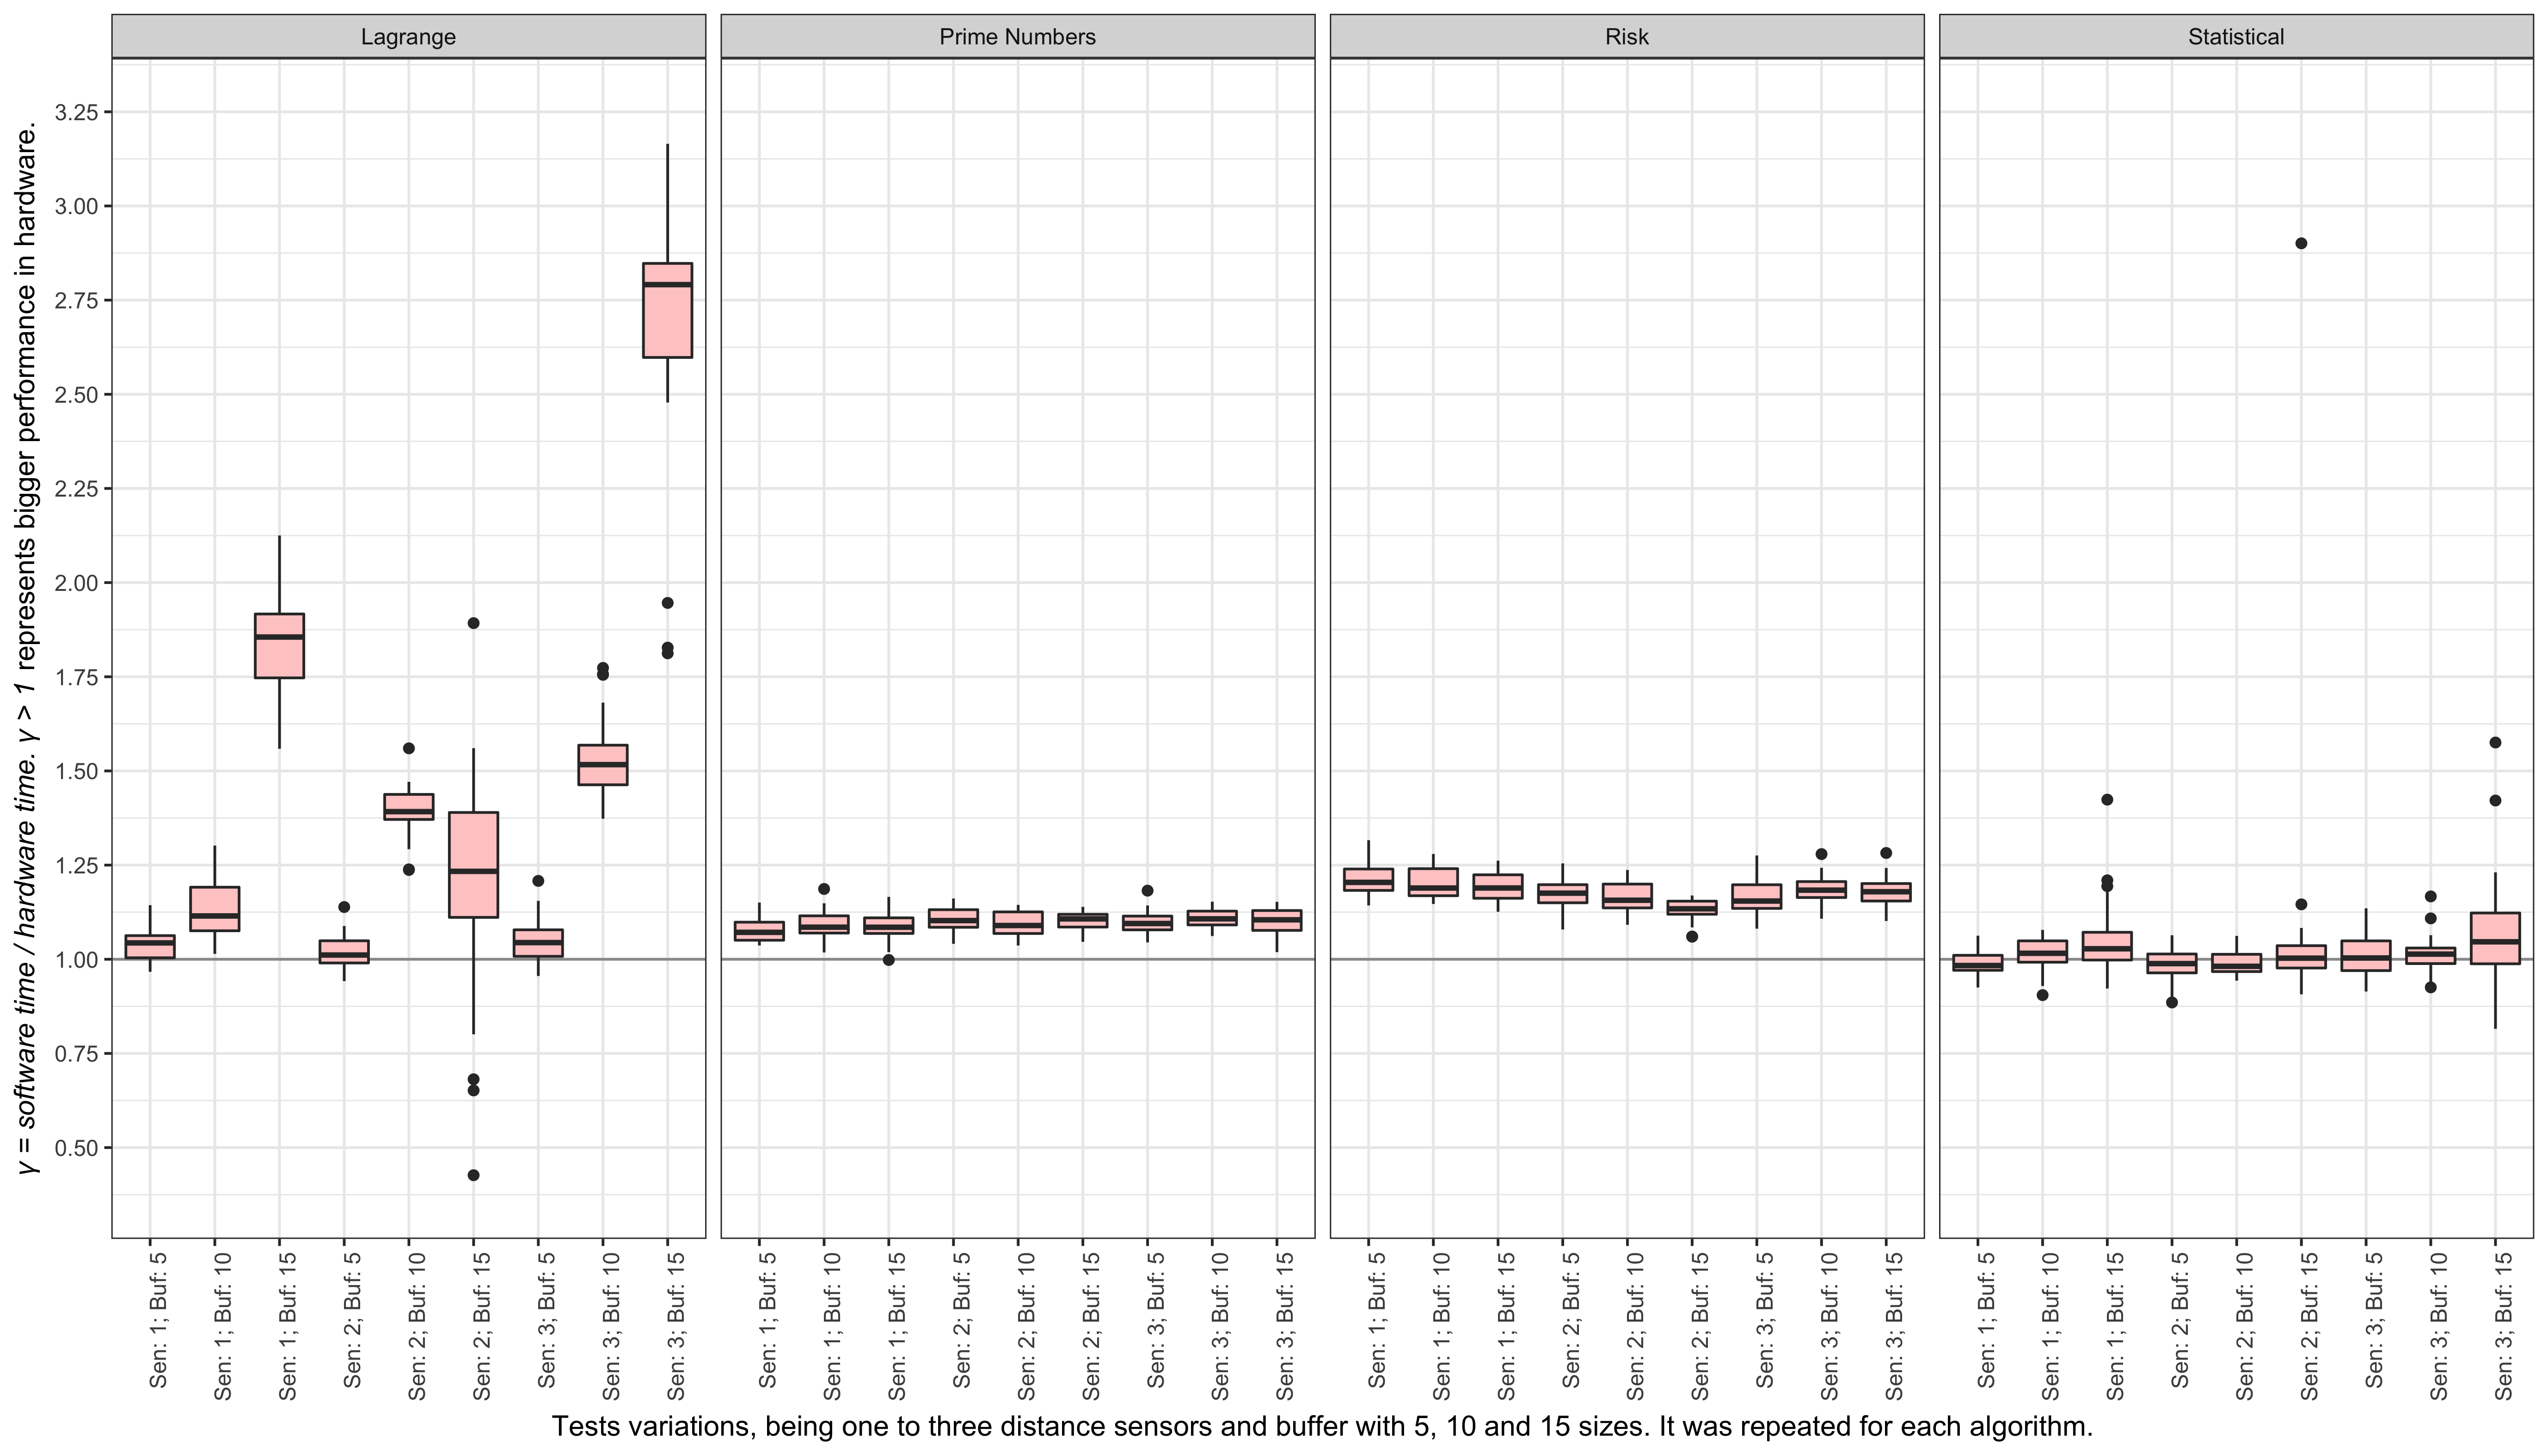
\includegraphics[width=1\textwidth]{img/performance.png}
            \caption{Graphic with the performance values of the 36 prototype variations, separated by candidate code. The values of $ \gamma > 1.0 $ show bigger performance in partitioned hardware than software.}
            
            \label{fig:performance}
        \end{figure*}
   
    
        %Além da Figura~\ref{fig:performance}, os valores médios também podem ser lidos pela Tabela~\ref{tab:performance}.
        %Cada linha desta representa um quadro da Figura~\ref{fig:performance}.
        %Como complemento, na última coluna tem-se uma média de desempenho de cada algoritmo em todas as suas variações de teste.
        Beyond the Figure~\ref{fig:performance}, the mean values also are shown by Table~\ref{tab:performance}.
        Each line represents a frame of Figure~\ref{fig:performance}.
        As a compliment, in the last column has a performance mean of each algorithm in all its test variations.
        
        \begin{table}[b]\centering
            \vspace{-1em}
            \scriptsize
            \raaa{1.0}
            %\raaa{0.9}
            \caption{Mean of Performance Analysis in its Variations}
            \begin{tabular}{@{}R{1.3em}R{1.6em}R{1.5em}R{1.5em}|R{1.6em}R{1.6em}R{1.6em}|R{1.5em}R{1.5em}R{1.5em}|c@{}}\toprule
                & \multicolumn{3}{c}{1 Sensor} & \multicolumn{3}{c}{2 Sensors} & \multicolumn{3}{c}{3 Sensors}& \\
                \cmidrule{2-11}
                \textit{Buffer} & 5 & 10 & 15 & 5 & 10 & 15 & 5 & 10 & 15 & $\bar{x}$ \\
                \midrule
                \Ss$_{St}$   & 0.989 & 1.013 & 1.052  & 0.982 & 0.992 & 1.069  & 1.009 & 1.011 & 1.08  & 1.022 \\
                \Ss$_{La}$   & 1.036 & 1.132 & 1.844  & 1.019 & 1.395 & 1.14   & 1.046 & 1.37  & 2.765 & 1.416 \\
                \Ss$_{PN}$   & 1.076 & 1.092 & 1.084  & 1.105 & 1.094 & 1.103  & 1.099 & 1.109 & 1.102 & 1.096 \\ 
                \Ss$_{Ri}$   & 1.212 & 1.203 & 1.195  & 1.17  & 1.161 & 1.132  & 1.168 & 1.183 & 1.179 & 1.178 \\
                \bottomrule
            \end{tabular}
            \label{tab:performance}
        \end{table}
        
        %Análise de performance
        % quase todos foram suuuuuuuucesssooooooooo 
        %Os resultados mostram que:
        The results show that:
        \begin{itemize}
            \item 
            %Os algoritmos Número Primo e Risco (\Ss$_{PN}$ e \Ss$_{Ri}$) obtiveram um ganho de desempenho considerável e estável, comparado com suas versões não particionadas, sendo em média $9,6\%$ e $17,8\%$ mais eficiente em suas tarefas;
            The Prime Number and Risk Algorithms (\Ss$_{PN}$ and \Ss$_{Ri}$) have a considerable and stable performance gain comparing with its versions non-partitioned, being meanly 9,6\% and 17,8\% more efficient in its tasks;
            
            \item 
            %Mesmo com o algoritmo Lagrange (\Ss$_{La}$) exibindo resultados não-estáveis nas variações como os de \Ss$_{PN}$ e \Ss$_{Ri}$, $87\%$ dos testes realizados obtiveram maior desempenho em \hardware.
            %Superando a versão em \software\ em $41,6\%$;
            Even with the Lagrange (\Ss$_{La}$) showing results not so stables in its variations as the \Ss$_{PN}$ and \Ss$_{Ri}$, 87\% of its tests had bigger performance in hardware.
            It overcame its software version in 41,6\%;
            
            \item 
            %O algoritmo Estatístico (\Ss$_{St}$) obteve três situações, na qual não utilizar o particionamento resultava em maior desempenho, sendo $45,5\%$ foram iguais ou melhores em \software.
            %São elas: [\textit{Sen} 1; \textit{Buf} 5], [\textit{Sen} 2; \textit{Buf} 5] e [\textit{Sen} 2; \textit{Buf} 10]. 
            %Entretanto, a média de todos os seus testes mostram que ainda assim foi $2,2\%$ mais eficiente em \hardware\ que \software.
            The Statistical (\Ss$_{St}$) obtained three situations, in which not using partitioning resulted in higher performance, being 45,5\% was equal or bigger in software.
            Are they: [\textit{Sen} 1; \textit{Buf} 5], [\textit{Sen} 2; \textit{Buf} 5] and [\textit{Sen} 2; \textit{Buf} 10]. 
            However, the mean of all its tests shows that they still were 2,2\% more efficient in hardware than software.
        \end{itemize}
    
    
        %\item 
        % Achismos
        %O baixo resultado de \Ss$_{St}$ já era esperado, pois este e todos os outros algoritmos não receberam nenhuma otimização em \hardware,\ nem em sua interface de comunicação.
        %O algoritmo Estático especificamente (Algoritmo \ref{alg:statistic}), é o único que realiza mais de uma leitura sobre os dados de \buffer\ via parâmetro, sendo as operações situadas nas linhas 3 e 5.
        %Este algoritmo é custoso, pois o uso de cada elemento de \buffer\ requer também uma comunicação entre \hs,\ solicitando o respectivo dado, criando uma sobrecarga no barramento e, consequentemente, a queda de desempenho pela sua espera.
        The low result of \Ss$_{St}$ was already expected because this and all the others algorithms neither received optimizations in hardware nor communications interface. 
        The \Ss$_{St}$ is explicitly the only that does more than one read over the buffer data via parameter, being the operations in lines 3 and 5 of Algorithm \ref{alg:statistic}.
        This algorithm is expensive, because the use of each buffer element also requires a hardware and software communication, requesting the respective data, making an overload and consequently, the performance decline.
        
        
        %resolvendo o problema
        %Este problema pode ser contornado de várias formas.
        %A mais simples seria utilizar uma memória interna no \hardware\ extra que, após a cópia de todos os valores do \buffer, pode-se operar lendo da sua própria memória.
        %\textit{Pipeline}, \textit{unroll} de \textit{loops} e protocolos de comunicação adequados são tipos de otimizações mais complexas, mas que poderiam resultar em melhora de desempenho, não aplicando só ao Estatístico, mas também todos os outros.
        This problem can be resolved in many ways.
        The most simple would be to use an internal memory in hardware that, after the copy, the buffer data to it, can operate reading of its memory.
        A pipeline, unroll loops, and better communications protocols also are types of optimizations more complexes, but that could result in performance enhancement, not applying just for Statistical, but all of the rest.
        